\documentclass[12pt]{chmullighw}
\usepackage{tikz}
\usepackage{tikz-qtree}
\usepackage{algorithm2e}
\usetikzlibrary{shapes,chains,fit,shapes,matrix}


% info for header block in upper right hand corner
\name{Chris Mulligan}
\uni{clm2186}
\class{COMS3137 Data Structures \& Algorithms}
\professor{Hershkop}
\assignment{Theory 3}
\duedate{October 27, 2013}

\lstset{language=Java, numbers=none, frame=l, captionpos=n}
\begin{document}
\problemlist{Theory 3} %Give us a nice big title
\begin{enumerate}

\item \begin{enumerate} \renewcommand{\labelenumii}{\alph{enumii}.}
    \item Chaining:

        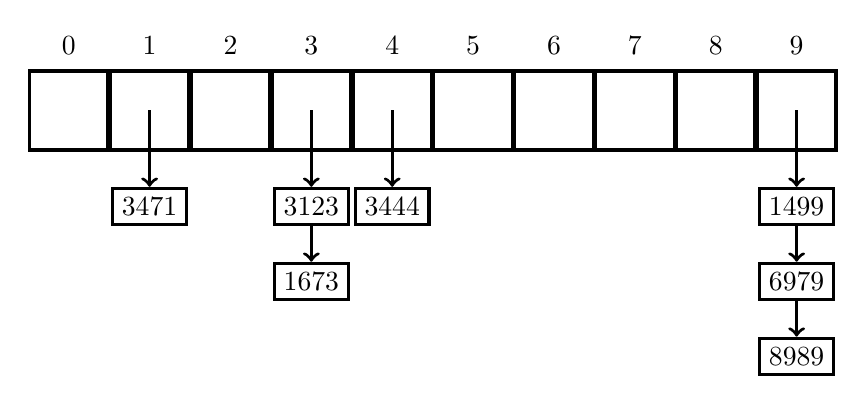
\begin{tikzpicture}
        \tikzstyle{every path}=[very thick]

        \edef\sizetape{1cm}
        \tikzstyle{ht}=[draw,minimum size=\sizetape]
        \tikzstyle{num}=[draw=none]
        \tikzstyle{value}=[draw]

        \begin{scope}[start chain=1 going right,node distance=-0.15mm]
        \foreach \x in {0, 1,...,9} {
            \node [on chain=1,ht] (\x) {};
        };
        \end{scope}

        %label the cells above
        \foreach \x in {0, 1,...,9} {
            \node [num,yshift=.3cm] at (\x.north) (\x_label) {$\x$};
        };

        \node[value, yshift=-.7cm] at (1.south) (3471) {3471};
        \draw[->] (1.center) -- (3471.north);

        \node[value, yshift=-.7cm] at (3.south) (3123) {3123};
        \draw[->] (3.center) -- (3123.north);
        \node[value, yshift=-.7cm] at (3123.south) (1673) {1673};
        \draw[->] (3123.south) -- (1673.north);

        \node[value, yshift=-.7cm] at (4.south) (3444) {3444};
        \draw[->] (4.center) -- (3444.north);
          
        \node[value, yshift=-.7cm] at (9.south) (1499) {1499};
        \draw[->] (9.center) -- (1499.north);
        \node[value, yshift=-.7cm] at (1499.south) (6979) {6979};
        \draw[->] (1499.south) -- (6979.north);
        \node[value, yshift=-.7cm] at (6979.south) (8989) {8989};
        \draw[->] (6979.south) -- (8989.north);
        \end{tikzpicture}

    \item Linear Probing:

        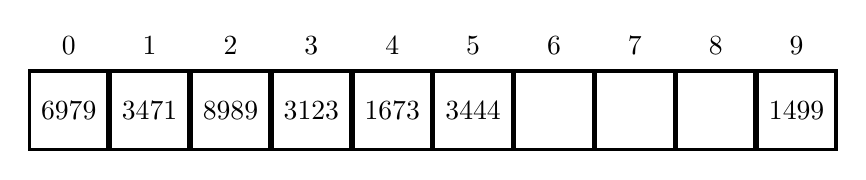
\begin{tikzpicture}
        \tikzstyle{every path}=[very thick]

        \edef\sizetape{1cm}
        \tikzstyle{ht}=[draw,minimum size=\sizetape]
        \tikzstyle{num}=[draw=none]
        \tikzstyle{value}=[draw]

        \begin{scope}[start chain=1 going right,node distance=-0.15mm]
        \node [on chain=1,ht] (0) {6979};
        \node [on chain=1,ht] (1) {3471};
        \node [on chain=1,ht] (2) {8989};
        \node [on chain=1,ht] (3) {3123};
        \node [on chain=1,ht] (4) {1673};
        \node [on chain=1,ht] (5) {3444};
        \node [on chain=1,ht] (6) {};
        \node [on chain=1,ht] (7) {};
        \node [on chain=1,ht] (8) {};
        \node [on chain=1,ht] (9) {1499};
        \end{scope}

        %label the cells above
        \foreach \x in {0, 1,...,9} {
            \node [num,yshift=.3cm] at (\x.north) (\x_label) {$\x$};
        };
        \end{tikzpicture}

    \item Quadratic Probing:

        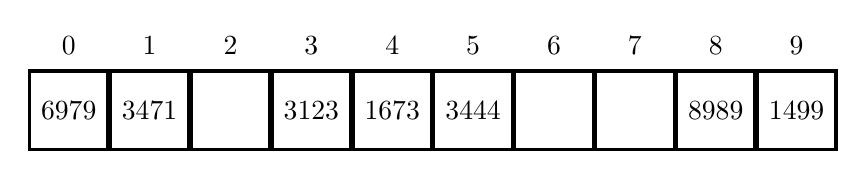
\begin{tikzpicture}
        \tikzstyle{every path}=[very thick]

        \edef\sizetape{1cm}
        \tikzstyle{ht}=[draw,minimum size=\sizetape]
        \tikzstyle{num}=[draw=none]
        \tikzstyle{value}=[draw]

        \begin{scope}[start chain=1 going right,node distance=-0.15mm]
        \node [on chain=1,ht] (0) {6979};
        \node [on chain=1,ht] (1) {3471};
        \node [on chain=1,ht] (2) {};
        \node [on chain=1,ht] (3) {3123};
        \node [on chain=1,ht] (4) {1673};
        \node [on chain=1,ht] (5) {3444};
        \node [on chain=1,ht] (6) {};
        \node [on chain=1,ht] (7) {};
        \node [on chain=1,ht] (8) {8989};
        \node [on chain=1,ht] (9) {1499};
        \end{scope}

        %label the cells above
        \foreach \x in {0, 1,...,9} {
            \node [num,yshift=.3cm] at (\x.north) (\x_label) {$\x$};
        };
        \end{tikzpicture}

    \item Second hash function $h_2(x) = 7 - (x \mod 7)$:

        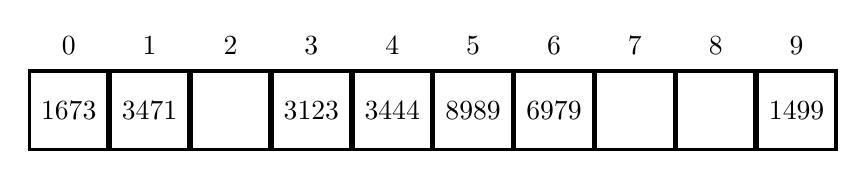
\begin{tikzpicture}
        \tikzstyle{every path}=[very thick]

        \edef\sizetape{1cm}
        \tikzstyle{ht}=[draw,minimum size=\sizetape]
        \tikzstyle{num}=[draw=none]
        \tikzstyle{value}=[draw]

        \begin{scope}[start chain=1 going right,node distance=-0.15mm]
        \node [on chain=1,ht] (0) {1673};
        \node [on chain=1,ht] (1) {3471};
        \node [on chain=1,ht] (2) {};
        \node [on chain=1,ht] (3) {3123};
        \node [on chain=1,ht] (4) {3444};
        \node [on chain=1,ht] (5) {8989};
        \node [on chain=1,ht] (6) {6979};
        \node [on chain=1,ht] (7) {};
        \node [on chain=1,ht] (8) {};
        \node [on chain=1,ht] (9) {1499};
        \end{scope}

        %label the cells above
        \foreach \x in {0, 1,...,9} {
            \node [num,yshift=.3cm] at (\x.north) (\x_label) {$\x$};
        };
        \end{tikzpicture}

\end{enumerate}


\item If in advance you knew the contents of a hash table you could potentially
avoid a collision, but it would be incredibly inefficient. Using perfect hashing
you have to calculate hashes and determine if anything collides. Then if they do
ever collide you would switch table size, or hash function, to prevent the
collision. However ultimately you'd end up doing substantially more work, and
likely wasting more memory, since we'd want our hash table to be approximately
$n^2$ to reduce the chance of collisions.

\newpage
\item Assuming this is a min heap, such that every parent is smaller than both
of its children.

%\Tree[.23 ]

%\Tree[.23 [.25 ]  \edge[draw=none];[.{} ] ]
After 23, 25, 14: \\
\Tree[.14 [.25 ] [.23 ] ]

%\Tree[.14 [.25 [.27 ] \edge[draw=none];[.{} ] ]
%          [.23 ] ]

%\Tree[.14 [.19 [.27 ] [.25 ] ]
%          [.23 ] ]
After 23, 25, 14, 27, 19, 18: \\
\Tree[.14 [.19 [.27 ] [.25 ] ]
          [.18 [.23 ] \edge[draw=none];[.{} ] ] ]

%\Tree[.14 [.19 [.27 ] [.25 ] ]
%          [.18 [.23 ] [.21 ] ] ]

%\Tree[.14 [.19 [.27 [.28 ] \edge[draw=none];[.{} ] ]
%               [.25 ] ]
%          [.18 [.23 ] [.21 ] ] ]
After 23, 25, 14, 27, 19, 18, 21, 28, 24: \\
\Tree[.14 [.19 [.24 [.28 ] [.27 ] ]
               [.25 ] ]
          [.18 [.23 ] [.21 ] ] ]

%\Tree[.14 [.19 [.24 [.28 ] [.27 ] ]
%               [.22 [.25 ] \edge[draw=none];[.{} ]] ]
%          [.18 [.23 ] [.21 ] ] ]

%\Tree[.14 [.19 [.24 [.28 ] [.27 ] ]
%               [.20 [.25 ] [.22 ] ] ]
%          [.18 [.23 ] [.21 ] ] ]
After 23, 25, 14, 27, 19, 18, 21, 28, 24, 22, 20, 17: \\
\Tree[.14 [.19 [.24 [.28 ] [.27 ] ]
               [.20 [.25 ] [.22 ] ] ]
          [.17 [.18 [.23 ] \edge[draw=none];[.{} ] ]
               [.21 ] ] ]

%\Tree[.14 [.19 [.24 [.28 ] [.27 ] ]
%               [.20 [.25 ] [.22 ] ] ]
%          [.17 [.18 [.23 ] [.24 ] ]
%               [.21 ] ] ]

%\Tree[.14 [.19 [.24 [.28 ] [.27 ] ]
%               [.20 [.25 ] [.22 ] ] ]
%          [.17 [.18 [.23 ] [.24 ] ]
%               [.21 [.26 ] \edge[draw=none];[.{} ] ] ] ]
Final:\\
\Tree[.14 [.19 [.24 [.28 ] [.27 ] ]
               [.20 [.25 ] [.22 ] ] ]
          [.15 [.18 [.23 ] [.24 ] ]
               [.17 [.26 ] [.21 ] ] ] ]

\newpage \item Chaining is one hash collision resolution strategy. Whenever an
element collides with an existing element, you create a linked list and append
the new element onto the old one. The advantages are that this is fairly
straight forward, you don't have to lazily delete, and a large number of
collisions in one position don't cause collisions in another. The downside is
that the linked lists may become arbitrarily long, and searching in them is slow
and unpredictable. Tracking linked list size will help know when to grow the
table and reduce chain sizes.

Another solution is cuckoo hashing, where a second hash table (or the second
half of a much larger hash table) is used. When a collision occurs one of the
entries is forced to move to the second table, where a different hash function
is used. There may be a cascade of collisions, but with reasonable sizes and
functions there will only rarely be a cycle. The biggest upside is that lookups
are very fast, with only 2 possible locations for every element. The downside is
that inserts are complex and expensive, and may require more memory to
implement. Resolving collisions in a relatively full hash table can become very
hard.

\item Duplicate items may not be properly detected in this scheme. If an
preliminary search isn't done to determine if the element is in the list at all,
by replacing the first lazily deleted element with a new element, we may be
introducing a duplicate.

Additionally whether it actually saves space or not depends on a number of
assumptions about the structure of the table, and what is meant by saving space.
The amount of memory consumed won't change, since hash tables are almost
universally implemented as arrays with a fixed size, unless the deleted item can
be freed, which is an independent question.

\item If we want a min heap, and we're using an array to store the heap we're
basically already done. A sorted list is a special case of a heap where all
levels are also sorted. This will be \BigO{n} to copy the elements into the
tree, and because we start with the min at the root, and every value we add is
at least as large as all previous elements, no element will ever have to bubble
up/down to maintain the heap property.

\item Insertion sort is stable, because it can easily choose to respect original
ordering when choosing where to place duplicates relative to each other.

Selection sort can be stable at the cost of additional runtime complexity.
Typically it's unstable because it simply swaps the original nth element with
the nth largest element in the unsorted portion of the list. However if you add
an additional check to verify that it always maintains the order of identical
items during a swap, it will be stable.

Bubble sort is stable, because it can view identical items as already in order,
so it won't every alter their relative ordering.

Merge sort is stable if coded properly. The merge simply has to bias toward the
earlier sublist in the case of equal values, and the sort becomes stable.

Heapsort is not stable, since establishing the heap property will break relative
ordering.

Quicksort is not stable generally, since the partition swapping can change
relative ordering. With care relative ordering may be preserved, at the cost of
substantial extra time (to check if there are other equal elements).

\item An AVL tree vs a Hashtable depends on the likely usage patterns.

AVL trees offer \BigO{\log n} inserts, finds, and deletes, which is reasonably
fast. The key feature of AVL trees are that because they're a BST the items are
maintained in order, permitting relatively easy ordered traversal of the list,
as well as getting the minimum and maximum values. They can also be more memory
efficient, depending on the memory overhead of the node structure, since the
only wasted space is the node overhead and pointers to the children.

Hashtables offer \BigO{1} inserts, finds, and deletes, which makes them much
faster for large ns. However they are unordered, and finding minimum and
maximums is \BigO{n}. Additionally they require extra space depending on the
load factor, generally at least double the actual number of elements. However
since there is no overhead per element the actual space usage of AVL and Hash
tables depends on implementation and language.

\item Huffman compression is \BigO{n log n}. Using a heap to build the tree
costs \BigO{n}, and taking the min each time costs \BigO{\log n}, for an overall
runtime of \BigO{n \log n}.

Decompression is simpler, each element is represented in the file, and each has
to be touched once, meaning it's at least \BigO{n}. Luckily with any efficient
lookup for the codes, say a perfect hash, lookup is \BigO{1}, for overall
runtime of \BigO{n} for decompression.

\item We know any arbitrary array can be converted to a heap in \BigO{n} steps
through the buildheap algorithm. To convert the min heap to a max heap we can
start at the leaves and check whether the heap property is satisfied, and if not
bubble up the larger element until it is. Overall this is \BigO{n}. 

It may be possible to have a \BigO{n} algorithm with a smaller constant multiple
by first reversing the list, so that it more closely resembles a max heap and
fewer bubble operations are required. However the big-O runtime would still be
\BigO{n}.

\end{enumerate} %end of questions
\end{document}
